
\captionsbrazil
\chapter{Tabelas}
\label{appendice_tables}

% ======= Tabela de genes sementes ==========
\begin{table}[]
\centering
\tiny
\caption{Tabela com os genes sementes do experimento original}
\label{table_original_seeds}
\begin{tabular}{@{}rlll@{}}
\toprule
\textbf{\textsl{Code 1}} & \textbf{GENE} &   \textbf{Description} & \textbf{Code 2} \\ \midrule
4524 & \textbf{MTHFR} & 5,10-methylenetetrahydrofolate reductase (NADPH) & 1p36.3 \\
5999 & \textbf{RGS4} & regulator of G-protein signaling 4 & 1q23.3 \\
5362 & \textbf{PLXNA2} & plexin A2 & 1q32.2 \\
27185 & \textbf{DISC1} & disrupted in schizophrenia 1 & 1q42.1 \\
7166 & \textbf{TPH1} & tryptophan hydroxylase 1 & 11p15.3-p14 \\
1815 & \textbf{DRD4} & dopamine receptor D4 & 11p15.5 \\
2900 & \textbf{GRIK4} & glutamate receptor, ionotropic, kainate 4 & 11q22.3 \\
1813 & \textbf{DRD2} & dopamine receptor D2 & 11q23 \\
9638 & \textbf{FEZ1} & fasciculation and elongation protein zeta 1 (zygin I) & 11q24.2 \\
4978 & \textbf{OPCML} & opioid binding protein/cell adhesion molecule-like & 11q25 \\
2904 & \textbf{GRIN2B} & glutamate receptor, ionotropic, N-methyl D-aspartate 2B & 12p12 \\
1610 & \textbf{DAO} & D-amino-acid oxidase & 12q24 \\
3356 & \textbf{HTR2A} & 5-hydroxytryptamine (serotonin) receptor 2A & 13q14-q21 \\
207 & \textbf{AKT1} & v-akt murine thymoma viral oncogene homolog 1 & 14q32.32|14q32.32 \\
23322 & \textbf{RPGRIP1L} & RPGRIP1-like & 16q12.2 \\
3240 & \textbf{HP} & haptoglobin & 16q22.1 \\
7157 & \textbf{TP53} & tumor protein p53 & 17p13.1 \\
6532 & \textbf{SLC6A4} & solute carrier family 6, member 4 & 17q11.1-q12 \\
348 & \textbf{APOE} & apolipoprotein E & 19q13.2 \\
3553 & \textbf{IL1B} & interleukin 1, beta & 2q14 \\
2571 & \textbf{GAD1} & glutamate decarboxylase 1 (brain, 67kDa) & 2q31 \\
91752 & \textbf{ZNF804A} & zinc finger protein 804A & 2q32.1 \\
2066 & \textbf{ERBB4} & v-erb-a erythroblastic leukemia viral oncogene homolog 4 & 2q33.3-q34 \\
1312 & \textbf{COMT} & catechol-O-methyltransferase & 22q11.21-q11.23|22q11.21 \\
2561 & \textbf{GABRB2} & gamma-aminobutyric acid (GABA) A receptor, beta 2 & 5q34 \\
1812 & \textbf{DRD1} & dopamine receptor D1 & 5q35.1 \\
2913 & \textbf{GRM3} & glutamate receptor, metabotropic 3 & 7q21.1-q21.2 \\
5649 & \textbf{RELN} & reelin & 7q22 \\
3084 & \textbf{NRG1} & neuregulin 1 & 8p12 \\
5533 & \textbf{PPP3CC} & protein phosphatase 3 (formerly 2B), catalytic subunit & 8p21.3 \\
267012 & *DAOA & D-amino acid oxidase activator & 13q33.2|13q34 \\
64067 & *NPAS3 & neuronal PAS domain protein 3 & 14q12-q13 \\
1139 & *CHRNA7 & cholinergic receptor, nicotinic, alpha 7 & 15q14 \\
5625 & *PRODH & proline dehydrogenase (oxidase) 1 & 22q11.21 \\
84062 & *DTNBP1 & dystrobrevin binding protein 1 & 6p22.3 \\
266553 & *OFCC1 & orofacial cleft 1 candidate 1 & 6p24.3 \\
63915 & *MUTED & muted homolog (mouse) & 6p25.1-p24.3 \\
6570 & *SLC18A1 & solute carrier family 18 (vesicular monoamine), member 1 & 8p21.3 \\ \bottomrule
\end{tabular}

\flushleft{Obs: durante a integração, apenas os 30 primeiros genes sementes possuíam correspondentes na rede \textsl{\textbf{PPI}}. Os 8 últimos genes (com o marcador \textsl{\textbf{*}})  não apresentaram integração com a rede \textsl{\textbf{PPI}}.

Fonte: Tabela gerada pelo autor.}
\end{table}

% ===========================================


% ========================== APENDICE SCRIPTS ======================

\chapter{Scripts}
\label{appendice_scripts}

\tiny
\label{CVV_script}
\begin{lstlisting}[caption={Script em Python para geração dos experimentos com remoção de mais de um gene semente.},label=getBlockStatic,language=Python]

class CrossValidationBased():
	def __init__(self):
		self.LEntrada = []  #Ex: [1,2,4,5,6]
		self.lenEntrada = 0 #Tamanho entrada
		self.LSaida = []    #Lista de saida
		self.k = 0          #iteracoes
		self.remocoes = 0   #Qtd Remocoes
		self.newLen = 0 
		self.removidas = []


	''' 
	 @params list {[]}	(Lista semente)
	 @params rem {int}	(% da lista a ser removida)
	 @params it {int}	(quantidade de listas a serem geradas)
	 ''' 
	def setData(self,list,rem,it):
		self.LEntrada = list
		self.k = it
		self.lenEntrada = len(self.LEntrada)
		self.remocoes = int(rem*self.lenEntrada)
		self.newLen = self.lenEntrada - self.remocoes
		self.result = []
		self.removidas = []
		
	def generateResult(self):
		self.result = []
		self.removidas = []
		while(self.k>0):
			self.LSaida = []
			LNRemovidas = self.LEntrada[:]
			novoLen = self.lenEntrada
			while(novoLen > self.remocoes):
				r = random.randrange(0,novoLen)
				self.LSaida.append(LNRemovidas[r])
				LNRemovidas.pop(r)
				novoLen -= 1

			self.result.append(self.LSaida)
			self.removidas.append(LNRemovidas)
			self.k -=1

    '''
    Retorna lista de conjuntos resultantes
    @returns self.result {[[]]}
    '''
	def getResult(self):
		return self.result

    '''
    Retorna lista de conjuntos removidos em cada agrupamento
    @returns self.removidas {[]}
    '''
	def getRemovidas(self):
		return self.removidas


\end{lstlisting}



\tiny
\label{shell_run_all}
\begin{lstlisting}[caption={Script em \textsl{Shell} para execução automatizada dos experimentos.},label=getBlockStatic,language=Shell]
#! /bin/bash
program="neri.py"
call_command="python"
params="--nodisplay run"
temp_archive_map="mapIn.txt"
processed="processed.txt"

while read line; do
	 $call_command $program $params $line
	echo $line >> $processed
done < $temp_archive_map

\end{lstlisting}



\chapter{Configuração do ambiente}
\label{appendice_ambient}

%Imagem - Arvore de arquivos
\begin{figure}[ht!]
\centering
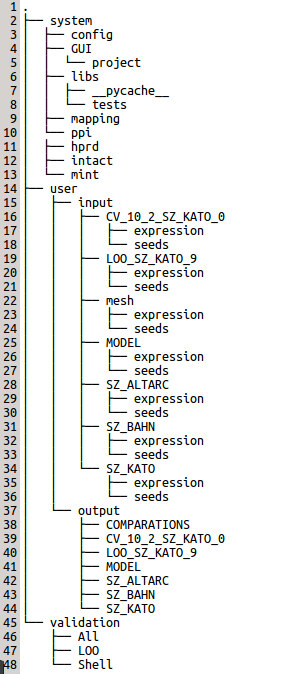
\includegraphics[width=80mm]{Images/tree.png}
\caption {Árvore de arquivos do programa \textsl{NERI}
\label{tree_files}}
\flushleft{
Árvore de arquivos 

Fonte: Produzido pelos autores.}
\end{figure}

